%  LaTeX support: latex@mdpi.com 
%  For support, please attach all files needed for compiling as well as the log file, and specify your operating system, LaTeX version, and LaTeX editor.

%=================================================================
\documentclass[mathematics,article,submit,pdftex,moreauthors]{Definitions/mdpi} 
% For posting an early version of this manuscript as a preprint, you may use "preprints" as the journal and change "submit" to "accept". The document class line would be, e.g., \documentclass[preprints,article,accept,moreauthors,pdftex]{mdpi}. This is especially recommended for submission to arXiv, where line numbers should be removed before posting. For preprints.org, the editorial staff will make this change immediately prior to posting.

%--------------------
% Class Options:
%--------------------
%----------
% journal
%----------
% Choose between the following MDPI journals:
% acoustics, actuators, addictions, admsci, adolescents, aerospace, agriculture, agriengineering, agronomy, ai, algorithms, allergies, alloys, analytica, animals, antibiotics, antibodies, antioxidants, applbiosci, appliedchem, appliedmath, applmech, applmicrobiol, applnano, applsci, aquacj, architecture, arts, asc, asi, astronomy, atmosphere, atoms, audiolres, automation, axioms, bacteria, batteries, bdcc, behavsci, beverages, biochem, bioengineering, biologics, biology, biomass, biomechanics, biomed, biomedicines, biomedinformatics, biomimetics, biomolecules, biophysica, biosensors, biotech, birds, bloods, blsf, brainsci, breath, buildings, businesses, cancers, carbon, cardiogenetics, catalysts, cells, ceramics, challenges, chemengineering, chemistry, chemosensors, chemproc, children, chips, cimb, civileng, cleantechnol, climate, clinpract, clockssleep, cmd, coasts, coatings, colloids, colorants, commodities, compounds, computation, computers, condensedmatter, conservation, constrmater, cosmetics, covid, crops, cryptography, crystals, csmf, ctn, curroncol, currophthalmol, cyber, dairy, data, dentistry, dermato, dermatopathology, designs, diabetology, diagnostics, dietetics, digital, disabilities, diseases, diversity, dna, drones, dynamics, earth, ebj, ecologies, econometrics, economies, education, ejihpe, electricity, electrochem, electronicmat, electronics, encyclopedia, endocrines, energies, eng, engproc, ent, entomology, entropy, environments, environsciproc, epidemiologia, epigenomes, est, fermentation, fibers, fintech, fire, fishes, fluids, foods, forecasting, forensicsci, forests, foundations, fractalfract, fuels, futureinternet, futureparasites, futurepharmacol, futurephys, futuretransp, galaxies, games, gases, gastroent, gastrointestdisord, gels, genealogy, genes, geographies, geohazards, geomatics, geosciences, geotechnics, geriatrics, hazardousmatters, healthcare, hearts, hemato, heritage, highthroughput, histories, horticulturae, humanities, humans, hydrobiology, hydrogen, hydrology, hygiene, idr, ijerph, ijfs, ijgi, ijms, ijns, ijtm, ijtpp, immuno, informatics, information, infrastructures, inorganics, insects, instruments, inventions, iot, j, jal, jcdd, jcm, jcp, jcs, jdb, jeta, jfb, jfmk, jimaging, jintelligence, jlpea, jmmp, jmp, jmse, jne, jnt, jof, joitmc, jor, journalmedia, jox, jpm, jrfm, jsan, jtaer, jzbg, kidney, kidneydial, knowledge, land, languages, laws, life, liquids, literature, livers, logics, logistics, lubricants, lymphatics, machines, macromol, magnetism, magnetochemistry, make, marinedrugs, materials, materproc, mathematics, mca, measurements, medicina, medicines, medsci, membranes, merits, metabolites, metals, meteorology, methane, metrology, micro, microarrays, microbiolres, micromachines, microorganisms, microplastics, minerals, mining, modelling, molbank, molecules, mps, msf, mti, muscles, nanoenergyadv, nanomanufacturing, nanomaterials, ncrna, network, neuroglia, neurolint, neurosci, nitrogen, notspecified, nri, nursrep, nutraceuticals, nutrients, obesities, oceans, ohbm, onco, oncopathology, optics, oral, organics, organoids, osteology, oxygen, parasites, parasitologia, particles, pathogens, pathophysiology, pediatrrep, pharmaceuticals, pharmaceutics, pharmacoepidemiology, pharmacy, philosophies, photochem, photonics, phycology, physchem, physics, physiologia, plants, plasma, pollutants, polymers, polysaccharides, poultry, powders, preprints, proceedings, processes, prosthesis, proteomes, psf, psych, psychiatryint, psychoactives, publications, quantumrep, quaternary, qubs, radiation, reactions, recycling, regeneration, religions, remotesensing, reports, reprodmed, resources, rheumato, risks, robotics, ruminants, safety, sci, scipharm, seeds, sensors, separations, sexes, signals, sinusitis, skins, smartcities, sna, societies, socsci, software, soilsystems, solar, solids, sports, standards, stats, stresses, surfaces, surgeries, suschem, sustainability, symmetry, synbio, systems, taxonomy, technologies, telecom, test, textiles, thalassrep, thermo, tomography, tourismhosp, toxics, toxins, transplantology, transportation, traumacare, traumas, tropicalmed, universe, urbansci, uro, vaccines, vehicles, venereology, vetsci, vibration, viruses, vision, waste, water, wem, wevj, wind, women, world, youth, zoonoticdis 

%---------
% article
%---------
% The default type of manuscript is "article", but can be replaced by: 
% abstract, addendum, article, book, bookreview, briefreport, casereport, comment, commentary, communication, conferenceproceedings, correction, conferencereport, entry, expressionofconcern, extendedabstract, datadescriptor, editorial, essay, erratum, hypothesis, interestingimage, obituary, opinion, projectreport, reply, retraction, review, perspective, protocol, shortnote, studyprotocol, systematicreview, supfile, technicalnote, viewpoint, guidelines, registeredreport, tutorial
% supfile = supplementary materials

%----------
% submit
%----------
% The class option "submit" will be changed to "accept" by the Editorial Office when the paper is accepted. This will only make changes to the frontpage (e.g., the logo of the journal will get visible), the headings, and the copyright information. Also, line numbering will be removed. Journal info and pagination for accepted papers will also be assigned by the Editorial Office.

%------------------
% moreauthors
%------------------
% If there is only one author the class option oneauthor should be used. Otherwise use the class option moreauthors.

%---------
% pdftex
%---------
% The option pdftex is for use with pdfLaTeX. If eps figures are used, remove the option pdftex and use LaTeX and dvi2pdf.

%=================================================================
% MDPI internal commands
\firstpage{1} 
\makeatletter 
\setcounter{page}{\@firstpage} 
\makeatother
\pubvolume{1}
\issuenum{1}
\articlenumber{0}
\pubyear{2022}
\copyrightyear{2022}
%\externaleditor{Academic Editor: Firstname Lastname}
\datereceived{} 
%\daterevised{} % Only for the journal Acoustics
\dateaccepted{} 
\datepublished{} 
%\datecorrected{} % Corrected papers include a "Corrected: XXX" date in the original paper.
%\dateretracted{} % Corrected papers include a "Retracted: XXX" date in the original paper.
\hreflink{https://doi.org/} % If needed use \linebreak
%\doinum{}
%------------------------------------------------------------------
% The following line should be uncommented if the LaTeX file is uploaded to arXiv.org
%\pdfoutput=1

%=================================================================
% Add packages and commands here. The following packages are loaded in our class file: fontenc, inputenc, calc, indentfirst, fancyhdr, graphicx, epstopdf, lastpage, ifthen, lineno, float, amsmath, setspace, enumitem, mathpazo, booktabs, titlesec, etoolbox, tabto, xcolor, soul, multirow, microtype, tikz, totcount, changepage, attrib, upgreek, cleveref, amsthm, hyphenat, natbib, hyperref, footmisc, url, geometry, newfloat, caption

%=================================================================
%% Please use the following mathematics environments: Theorem, Lemma, Corollary, Proposition, Characterization, Property, Problem, Example, ExamplesandDefinitions, Hypothesis, Remark, Definition, Notation, Assumption
%% For proofs, please use the proof environment (the amsthm package is loaded by the MDPI class).

%=================================================================
% Full title of the paper (Capitalized)
\Title{Optimization of Turbulence Model Parameters Using the Global Search Method Combined with Machine Learning}

% MDPI internal command: Title for citation in the left column
\TitleCitation{Optimization of Turbulence Model Parameters Using the Global Search Method Combined with Machine Learning}

% Author Orchid ID: enter ID or remove command
\newcommand{\orcidauthorA}{0000-0001-5273-2471} % Add \orcidA{} behind the author's name
\newcommand{\orcidauthorB}{0000-0002-8736-0652} % Add \orcidB{} behind the author's name
\newcommand{\orcidauthorC}{0000-0002-0722-6884} % Add \orcidC{} behind the author's name

\newcommand{\orcidauthorD}{0000-0002-5771-4114} % Add \orcidD{} behind the author's name
\newcommand{\orcidauthorE}{0000-0001-5525-5180} % Add \orcidF{} behind the author's name
\newcommand{\orcidauthorF}{0000-0001-9568-7121} % Add \orcidG{} behind the author's name

% Authors, for the paper (add full first names)
%\Author{Firstname Lastname $^{1,\dagger,\ddagger}$\orcidA{}, Firstname Lastname $^{2,\ddagger}$ and Firstname Lastname $^{2,}$*}
\Author{Konstantin Barkalov $^{1}$\orcidA{}, Ilya Lebedev $^{1}$\orcidB{}, Marina Usova$^{1}$\orcidC{}, Daria Romanova$^{2,4}$\orcidD{}, Daniil~Ryazanov$^2$\orcidF{} and Sergei~Strijhak$^{2,3,}$*\orcidE{}}

%\longauthorlist{yes}

% MDPI internal command: Authors, for metadata in PDF
%\AuthorNames{Firstname Lastname, Firstname Lastname and Firstname Lastname}
\AuthorNames{Konstantin Barkalov, Ilya Lebedev, Marina Usova, Daria Romanova, Daniil~Ryazanov and Sergei~Strijhak}

% MDPI internal command: Authors, for citation in the left column
%\AuthorCitation{Lastname, F.; Lastname, F.; Lastname, F.}
\AuthorCitation{Barkalov, K.; Lebedev, I.; Usova, M.; Romanova, D.; Ryazanov, D.; Strijhak, S.}
% If this is a Chicago style journal: Lastname, Firstname, Firstname Lastname, and Firstname Lastname.

% Affiliations / Addresses (Add [1] after \address if there is only one affiliation.)
%\address{%
%$^{1}$ \quad Affiliation 1; e-mail@e-mail.com\\
%$^{2}$ \quad Affiliation 2; e-mail@e-mail.com}
\address{%
$^{1}$ \quad Department of Mathematical Software and Supercomputing Technologies, Lobachevsky University, 603022 Nizhni Novgorod, Russia; konstantin.barkalov@itmm.unn.ru (K.B.), ilya.lebedev@itmm.unn.ru (I.L.), marina.usova@itmm.unn.ru (M.U.)\\
$^{2}$ \quad Institute for System Programming of the Russian Academy of Sciences, 109004, Moscow, Russia; ryazanov@ispras.ru (D.Ryaz.), romanovadi@ispras.ru (D.Rom.)\\
$^{3}$ \quad Moscow Aviation Institute, 125993, Moscow, Volokolamskoe shosse, 4; s.strijhak@ispras.ru (S.S.)\\
$^{4}$ \quad Lomonosov Moscow State University, 119991, Moscow, Russia; romanovadi@gmail.com (D.Rom.)}

% Contact information of the corresponding author
%\corres{Correspondence: e-mail@e-mail.com; Tel.: (optional; include country code; if there are multiple corresponding authors, add author initials) +xx-xxxx-xxx-xxxx (F.L.)}
\corres{Correspondence: Sergei Strijhak s.strijhak@ispras.ru;}

% Current address and/or shared authorship
%\firstnote{Current address: Affiliation 3.} 
%\secondnote{These authors contributed equally to this work.}
% The commands \thirdnote{} till \eighthnote{} are available for further notes

%\simplesumm{} % Simple summary

%\conference{} % An extended version of a conference paper

% Abstract (Do not insert blank lines, i.e. \\) 
\abstract{The paper considers the slope flow simulation and the problem of finding the optimal parameter values of this mathematical model. The slope flow is modeled using the finite volume method applied to the Reynolds-averaged Navier–Stokes equations with closure in the form of the $k-\omega\ SST$ turbulence model. The optimal values of turbulence model coefficients for free surface gravity multiphase flows were found using the global search algorithm. Calibration was performed to increase the similarity of the experimental and calculated velocity profiles. The Root Mean Square Error (RMSE) of derivation between the calculated flow velocity profile and the experimental one is considered as the objective function in the optimization problem. The calibration of turbulence model coefficients for calculating the free surface flows on test slopes using the multiphase model for interphase tracking has not been performed earlier. To solve the multi-extremal optimization problem arising from the search for the minimum of the loss function for the flow velocity profile, we apply a new optimization approach using a Peano curve to reduce the dimensionality of the problem. To speed up the optimization procedure, the objective function was approximated using an artificial neural network. Thus, an interdisciplinary approach was applied which allowed the optimal values of six turbulence model parameters to be found using OpenFOAM and Globalizer software.}

% Keywords
\keyword{global optimization; artificial neural network; function approximation; finite volume method; CFD; OpenFOAM; interFoam} 

% The fields PACS, MSC, and JEL may be left empty or commented out if not applicable
%\PACS{J0101}
%\MSC{}
%\JEL{}

%%%%%%%%%%%%%%%%%%%%%%%%%%%%%%%%%%%%%%%%%%
% Only for the journal Diversity
%\LSID{\url{http://}}

%%%%%%%%%%%%%%%%%%%%%%%%%%%%%%%%%%%%%%%%%%
% Only for the journal Applied Sciences
%\featuredapplication{Authors are encouraged to provide a concise description of the specific application or a potential application of the work. This section is not mandatory.}
%%%%%%%%%%%%%%%%%%%%%%%%%%%%%%%%%%%%%%%%%%

%%%%%%%%%%%%%%%%%%%%%%%%%%%%%%%%%%%%%%%%%%
% Only for the journal Data
%\dataset{DOI number or link to the deposited data set if the data set is published separately. If the data set shall be published as a supplement to this paper, this field will be filled by the journal editors. In this case, please submit the data set as a supplement.}
%\datasetlicense{License under which the data set is made available (CC0, CC-BY, CC-BY-SA, CC-BY-NC, etc.)}

%%%%%%%%%%%%%%%%%%%%%%%%%%%%%%%%%%%%%%%%%%
% Only for the journal Toxins
%\keycontribution{The breakthroughs or highlights of the manuscript. Authors can write one or two sentences to describe the most important part of the paper.}

%%%%%%%%%%%%%%%%%%%%%%%%%%%%%%%%%%%%%%%%%%
% Only for the journal Encyclopedia
%\encyclopediadef{For entry manuscripts only: please provide a brief overview of the entry title instead of an abstract.}

%%%%%%%%%%%%%%%%%%%%%%%%%%%%%%%%%%%%%%%%%%
\begin{document}

\section{Introduction}

Climate change is accompanied by dangerous natural phenomena that are becoming more and more frequent. These phenomena inevitably affect human life and daily activities.  Research into these issues involves mathematical modeling and analysis of geophysical data as well as data from numerical and field experiments. The current trend in geodata analysis is associated with the use of machine learning algorithms and artificial neural networks.

Landslides, mudflows, and avalanches are classified as dangerous geological phenomena. These are slope processes associated with the separation of rocks, their movement along the slope under the influence of gravity and leading to irreversible changes in the relief. The study of the descent of landslides, mudflows, and avalanches as well as their prediction and detection are highly relevant due to the impact of these dangerous phenomena on human life and urban infrastructure. Landslides are distinguished according to the main causes of their occurrence. These are: abrasive, erosional, anthropogenic, and natural/anthropogenic. According to the mechanism of displacement, block landslides, shear, stretching, and liquefaction landslides are classified, respectively \cite{Pendin2015}.

Data show that between January 2004 and December 2016, landslides killed about 56 thousand of people in a little then 5 thousand incidents. The spatial distribution of landslides is uneven, with Asia as the predominant geographic area \cite{Froude2018}.

A large number of landslides, avalanches, and mudflows occur in European countries (Switzerland, Austria, Italy, France, and Iceland). Similar dangerous phenomena occur in Russia, for example, in Krasnodar Territory of the Russian Federation and in  North Caucasus due to heavy rainfalls in these regions where mountainous terrain is present and in connection with the development of the territory (linear and areal objects) in recent years \cite{hungr2005landslide}.  The amount of precipitation was outstanding in the above territories of Russia (Sochi, Krasnaya Polyana) in 2021. This led to the flooding of mountain rivers and increased the risk of slope flows. Catastrophic descents of mudflows occured resulting in damage to road equipment and blockage of roadways \cite{Harch2020}.

Mudflows are one of the most complex exogenous geological processes, which integrate the actions of other geological processes. The mudflow is a complex heterogeneous structure consisting of liquid and solid components. The solid fraction consists of mineral particles, which are nonuniform from the granulometric viewpoint.

%The most well-known landslide problem involves assessing the stability of a landslide slope for static conditions and seismic impact. Modeling the descent of the slope flow allows predicting the destruction caused by this phenomenon, correctly locating protective structures and vital objects.

The most well-known landslide problem involves assessing the stability of a landslide slope for static conditions and seismic impact. Modeling the descent of the slope flow makes it possible to predict the damage caused by this phenomenon and to correctly locate the protective structures and vital objects. Such problems are solved using the finite difference method \cite{Bernander2016}, the finite volume method \cite{liu2007application}, the discrete elements method \cite{Liu2020}, the cellular automata method  \cite{piegari2006cellular}, and hybrid methods. The mudflows can be modeled using a two-fluid model based on the Volume of Fluid model \cite{Hirt1981}. The methods listed above are implemented in various commercial and open source software packages MN2D \cite{Naaim2002}, TITAN2D \cite{Pitman2003}, and RAMMS.

Previously, the study of avalanches was carried out using computational fluid dynamics methods for Newtonian fluids and analysis of observation data including the historical data on avalanches in Japan \cite{Oda2011, Yamaguchi2017}. Similar work was carried out on avalanches in Switzerland, Austria, and Italy. A series of works on the study of avalanches using laboratory experiment in special trays and measuring equipment for studying avalanches in Iceland were carried out at the University of Iceland  \cite{IceThesKatr, IceThesJon}. An experiment with the descent of a snow-water stream in Davos, Switzerland was described in \cite{Jaedicke2006}. Measurements were made for the flow depth for a dry snow avalanche and for a snow-water flow.

Cheng et al. \cite{Cheung2011} used Bayesian analysis to calibrate the coefficients of the Spalart-Allmaras turbulence model to correct model deficiencies and reproduce the profile of a turbulent boundary layer over a flat plate. Among similar works, the coefficients were already calibrated in the $k-\varepsilon$ turbulence model when studying the process of the propagation of impurities in the process of urban development \cite{Guillas2014}.

Bayesian analysis is often used to calibrate the RANS closures turbulence models to improve forecast accuracy without losing computational efficiency (as was done for $k-\varepsilon$ model with Launder-Sharma damping functions, $k-\omega$ Wilcox model, Spalart-Allmaras and Baldwin-Lomax models \cite{Edeling2014a,Edeling2014b}). De Zordo-Banliat et al. applied Bayesian analysis to compressor cascades to obtain a set of calibrated turbulence model parameters due to the inadequacy of the original model \cite{deZordoBanliat2020}.

Kotaro Matsui et al. \cite{Matsui2021} proposed a new set of calibrated coefficients that improved the ability of the Spalart-Allmaras model to predict compressor cascade flow angular separation. A comprehensive review of turbulence model uncertainties is given in the paper of Xiao and Cinnella \cite{Xiao2019}.


A comprehensive analysis of climatic, geological, and hydrological data was applied to model and predict the slope flows. In the scope of recent trends, huge streams of data received from satellites, from the experiments, and from mathematical modeling are processed using machine learning, which makes it possible to develop efficient models of these processes \cite{GeoML, Ma2020}.

Methods based on convolutional neural networks (CNN) are able to extract stable spatial and spectral features \cite{Maggiori2017}. The combination of satellite image and topographic data can be used to generalize the extracted features in order to identify the slope flows in the satellite images \cite{Qin2021, Prakash2021}.

The slope flow model, as a rule, includes several parameters, the values of which cannot be specified in advance but can be selected based on the consistency of the numerical results with the experimental data available. Such a problem is a global optimization problem with a black box objective function because the specific type of the objective function is not known, there exists only the algorithm for calculating its values.

The complexity of the phenomena and processes under study is reflected in the complexity of the corresponding mathematical models and numerical methods for their analysis. Currently, the main (and often the only possible) tool for such an analysis is supercomputer modeling of the object behavior. Open source software is used widely for this purpose. OpenFOAM (an open platform for numerical modeling of continuum mechanics problems) is a well-known example of open source software of this kind \cite{Weller1998}. 

%ННГУ
% Если будет предыдущая связка, то вот этот абзац можно и опустить, и начать - со следующего,
The growing performance of modern supercomputer systems goes in parallel with complication of mathematical models of the processes considered that makes performing even a single model calculation (a \textit{trial}) a computation-costly operation. Consequently, the choice of the optimal values of the model parameters in reasonable time cannot be completed by trying all possible variants by the grid method, i.e. by search on some regular grid in the range of variation of the parameters. Impossibility of performing a large number of search trials requires applying efficient search algorithms, which would provide an acceptable estimate of a problem solution at a relatively small number of trials using available computational resources.

%ННГУ - начать можно отсюда
It is worth noting that most existing methods for finding the optimum of time-consuming black-box functions have some drawbacks. Gradient-based algorithms cannot be used in many cases just because the derivatives of an objective function are unknown while the finite-difference approximations of these derivatives are too computationally costly. At the same time, in general, gradient-based methods only allow finding a locally optimal solution to the problem.
Classical direct search methods, which don't require the derivatives, e.g. the Nelder-Mead method \cite{NelderMead} or the Hooke-Jeeves method \cite{HookJeeves}, are also local. As a rule, the application of these methods for solving global optimization problems involves several restarts from random grid nodes,  which requires a large number of trials. 

Deterministic methods of the Lipschitz global optimization, such as DIRECT \cite{Jones2009}, non-uniform coverages method \cite{Evtushenko2009, Evtushenko2013}, diagonal \cite{Sergeyev2017}, and simplicial \cite{Zilinskas2014} methods guarantee (in the limit) convergence to the global solution of the problem but may require a large number of search trials.
Finally, heuristic methods, e.g. differential evolution or simulated annealing, also require a very large amount of computations of the functions to obtain good estimates of the solutions in global optimization problems and at the same time lose in quality to the deterministic algorithms \cite{Sergeyev2018,Kvasov2018}.

So far, direct application of optimization algorithms to search for the minima of the time-consuming function may appear too computation-costly when a single trial takes much computation time. 
A well known method to overcome this problem is to construct an approximation of the objective function (also known as a response surface model or a metamodel or a surrogate model). Computing its values is a computationally inexpensive operation. The approximation is used further to find the minimum.
There are many variants of constructing the approximations for multivariate functions. These are various interpolation methods utilizing polynomials, splines, radial basis functions, Kriging, as well as various regression models. Many of these algorithms are used in the development of global optimization methods.

For example, the use of the radial basis functions has been considered in detail in \cite{Gutmann2001,Regis2005}. In \cite{Jones1998,UrRehman2014,Ollar2017_1}, Kriging-based methods have been proposed. A novel approach to constructing the metamodels and trust-region methods based on these ones has been presented in \cite{Polynkin2012,Ollar2017_2,Toropov2018}. 

In the present study, we used an efficient global search algorithm (GSA) \cite{Strongin2000,Sergeyev2013} for solving the Lipschitz global optimization problems combined with function approximations based on the regression models. At the first search stage, GSA worked with the objective function as a direct method. Then, an approximation of the objective function was constructed using the accumulated information. This approximation was used at the second stage of the search.
To construct the approximations, we applied Neural Network Regression (NNR).

To study the parameters of slope flows, it is advisable to use interdisciplinary approaches from the fields of computational and experimental hydrodynamics, optimization theory, parallel computing and neural networks. This paper uses the results of an experiment in a chute with a different angle of inclination, a mathematical model for modeling a two-phase flow, global optimization methods and an artificial neural network. The mathematical model is based on the averaged Reynolds equations and a two-parameter turbulence model. 

The turbulence model $k-\omega\ SST$ contains a number of constants calibrated for canonical flows in pipes and channels, air flow around various profiles, etc. \cite{LaunderSpalding1974, Tahry1983, LaunderMorseRodiSpaldiug1972}. Calibration of turbulence model coefficients was not carried out for calculating the free surface flows on slopes using the multiphase model for interphase tracking was performed. In this work, the coefficients of the $k-\omega\ SST$ turbulence model were optimized for calculating the turbulent fluid flow in the chute.

The main part of the paper has the following structure. 
Section 2 contains a description of the experiment. Section 3 describes the mathematical model of turbulent two-phase flows. Section 4 contains the details of numerical methods. 
Section 5 describes the results of numerical experiments. 
Section 6 concludes the paper. Nomenclature and list of abbreviations are presented in Appendix \ref{app}.


%%%%%%%%%%%%%%%%%%%%%%%%%%%%%%%%%%%%%%%%%%
\section{Inclined Chute Experiment }

To study slope flow parameters, experimental setups were used. The objects of study were such measurements as flow depth, flow velocity, and force of interaction with an obstacle. In our study, the velocity profile was studied.

An experimental setup at the Research Institute of Mechanics, Lomonosov Moscow State University \cite{fluids7030111} was used for this purpose. To carry out the calibration, a turbulent flow in an inclined chute was studied. Three different angles of inclination were used during the work. The chute had a simple rectangular geometry 1~m long, 12~cm wide and 10~cm high. The section of the chute to be examined was between two points of velocity and depth measurements located at the distances of 23~cm and 82~cm from the top side of chute. The schematic diagram of the experimental setup is shown in Figure~\ref{NIIMexLinearUProfileInlet}. Tap water was used in the experiment.

\begin{figure}[H]
\begin{center}
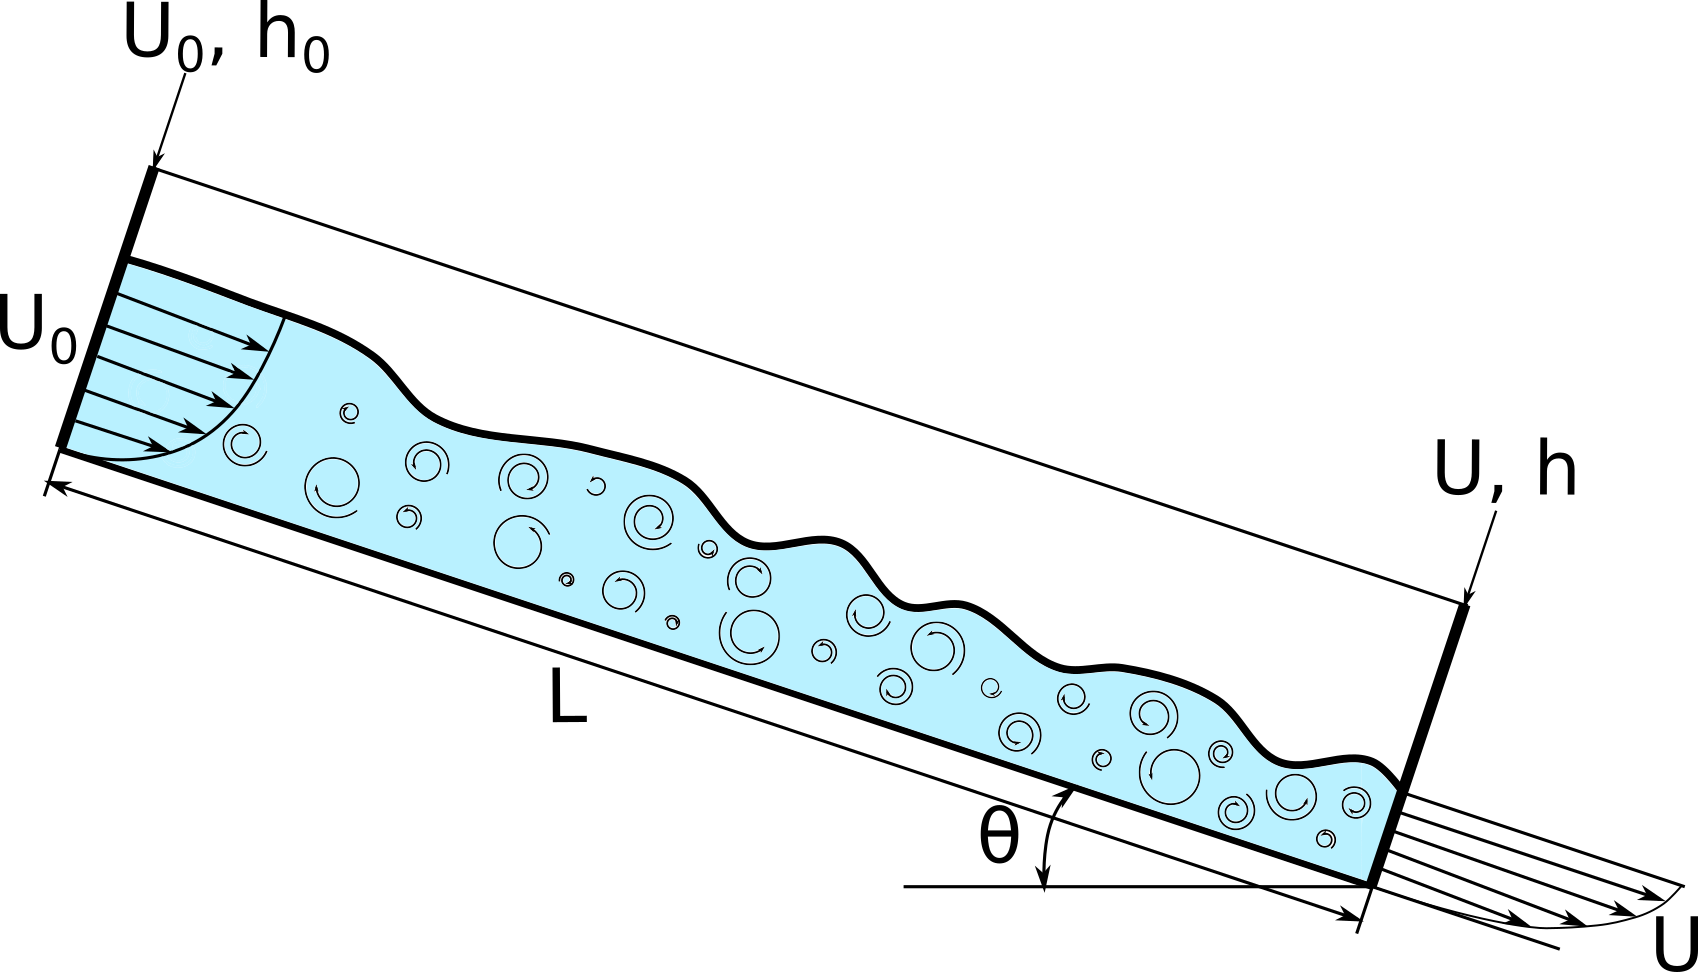
\includegraphics[width=10.5 cm]{NIIMexLinearUProfileInlet.png}
\caption{Schematic diagram of the experimental chute.\label{NIIMexLinearUProfileInlet}}
\end{center}
\end{figure}   
\unskip

%Было проведено 3 серии экспериментов, в которых менялся угол наклона склона, начальная глубина потока, начальный профиль потока, как показано в таблице \ref{tabNIIMexLinear}
Three series of experiments were performed; the initial flow profile, the initial flow depth, the slope angle were varied as shown in Table~\ref{tabNIIMexLinear}, where $u_0$ is the depth-averaged velocity, $h_0$ is the flow depth, $\theta$ is the slope inclination angle.

%\begin{table}[H]
%	\caption{Параметры расчётов}
%	\label{tabNIIMexLinear}
%	\begin{center}
%		\begin{tabular}{ | c | c | c | } 
%			\hline
%			$u_0$ среднее по глубине, м/с & $h_0$, мм & $\theta$\\
%			\hline
%			1.63 & 4.20 & 25$^\circ$\\
%			2.00 & 4.95 & 28$^\circ$\\
%			1.78 & 3.45 & 33$^\circ$\\
%			\hline
%		\end{tabular}
%	\end{center}
%\end{table}

\begin{table}[H] 
\caption{Parameters of the experiments.\label{tabNIIMexLinear}}
\newcolumntype{C}{>{\centering\arraybackslash}X}
\begin{tabularx}{\textwidth}{CCC}
\toprule
    \textbf{$\boldsymbol{u_0}$, m/s}	&    \textbf{$\boldsymbol{h_0}$, mm}	&     \textbf{$\boldsymbol{\theta}$}\\
\midrule
	1.63 & 4.20 & 25$^\circ$\\
	2.00 & 4.95 & 28$^\circ$\\
	1.78 & 3.45 & 33$^\circ$\\
\bottomrule
\end{tabularx}
\end{table}
\unskip

%%%%%%%%%%%%%%%%%%%%%

%ННГУ

\section{Mathematical model}\label{math_model}

%Для расчёта эксперимента поставленного в НИИ Механики МГУ используются осреднённые по Рейнольдсу уравнения Навье-Стокса. Для получения значений тензора напряжений Рейнольдса используется замыкание в виде $k-\omega\ SST$ модели турбулентности. Положение свободной поверхности потока определяется с использованием метода объёма жидкости VOF (Volume Of Fluid), предложенного Хиртом и Николсом в 1981 году \cite{HirtNichols1981}. В данном методе используется величина объёмной доли фазы воды $\alpha$ в ячейке для определения свободной поверхности таким образом, что при $\alpha>0.6$ считается что ячейка заполнена жидкостью, в противном случае~--- воздухом.
The Reynolds-averaged Navier-Stokes equations \cite{Navier,Stokes,Reynolds} were used to model the experiment carried out at the Research Institute of Mechanics of Lomonosov Moscow State University. The $k-\omega\ SST$ turbulence model \cite{Menter1993, Menter1994} was used to obtain the values of the Reynolds stress tensor. The position of the free surface of the flow is determined using the VOF (Volume Of Fluid) method suggested by C.W.~Hirt and B.D.~Nichols in 1981 \cite{HirtNichols1981}. In this method, the volume fraction of water phase $\alpha$ in the cell is used to determine the free surface so that if $\alpha>0.6$, the cell is considered to be filled with liquid, otherwise --- to be filled with air.

%Течение в экспериментальной у становке описывается системой из пяти уравнений. Это уравнения Навье-Стокса, осреднённые по Рейнольдсу (уравнение неразрывности и уравнение сохранения импульса). Так же в систему входит уравнение переноса объёмной доли фазы для отслеживания межфазной границы. Замыкают систему уравнения сохранения для турбулентной кинетической энергии и специальной диссипации турбулентной кинетической энергии, которые используются для вычисления напряжений Рейнольдса, возникающих при осреднении уравнений Навье-Стокса.
The flow in the experimental setup is described by a system of five equations \eqref{vofKWSST}. These are the Reynolds-averaged Navier-Stokes equations (continuity equation and momentum conservation equation). The system also includes a transfer equation for the phase volume fraction to track the interface. The system of equations is closed by two equations of conservation of turbulent kinetic energy and a special dissipation of turbulent kinetic energy, which are used to calculate the Reynolds stresses that arise when averaging the Navier-Stokes equations.

\begin{linenomath}
\begin{equation}
	\label{vofKWSST}
	\left\{
		\begin{aligned}
			&\boldsymbol{\nabla} \cdot \bar{\boldsymbol{u}} = 0,\\
			&\frac{\partial \alpha}{\partial t} + \boldsymbol{\nabla} \cdot (\bar{\boldsymbol{u}} \alpha) = 0,\\
			&\frac{\partial (\rho \bar{\boldsymbol{u}})}{\partial t} + \boldsymbol{\nabla} \cdot (\rho \bar{\boldsymbol{u}} \bar{\boldsymbol{u}}) = -\boldsymbol{\nabla} \bar{p} + \boldsymbol{\nabla} \cdot \bar{\boldsymbol{\tau}} + \rho \bar{\boldsymbol{f}},\\
			&\frac{\partial (\rho k)}{\partial t} + \boldsymbol{\nabla} \cdot (\rho \bar{\boldsymbol{u}} k) = \widetilde{P}_k - \beta^*\rho k \omega + \boldsymbol{\nabla} \cdot \left( (\mu + \alpha_k \mu_t) \boldsymbol{\nabla} k \right),\\
			&\frac{\partial (\rho \omega)}{\partial t}  + \boldsymbol{\nabla} \cdot ( \rho \bar{\boldsymbol{u}} \omega) = \gamma \rho \dot{s}^2 - \beta \rho \omega^2 + \boldsymbol{\nabla} \cdot \left( (\mu + \alpha_\omega \mu_t) \boldsymbol{\nabla} \omega \right) + \\
			&2 (1 - F_1) \rho \alpha_{\omega 2} \frac{1}{\omega} \boldsymbol{\nabla} k \cdot \boldsymbol{\nabla} \omega.
		\end{aligned}
	\right.
\end{equation}
\end{linenomath}

%Здесь $\boldsymbol{u}$~--- скорость смеси; $\alpha$~--- объёмная доля выбранной фазы; $\rho$~--- плотность смеси, рассчитываемая по принципу весового среднего; $\bar{\boldsymbol{\tau}} = 2 \mu_{eff} \bar{\boldsymbol{s}}$~--- тензор напряжений, выраженный через тензор скоростей деформации $\bar{\boldsymbol{s}}$, горизонтальной чертой над буквами обозначается осреднение по Рейнольдсу; $\mu_{eff} = \mu + \mu_t$~--- эффективный коэффициент вязкости, сумма молекулярной вязкости и турбулентной, последняя вычисляется по формуле $\mu_t = \rho a_1 k / \max(a_1 \omega,\ b_1 \dot{s} F_2)$; $\bar{p}$~--- давление; $\bar{\boldsymbol{f}}$~--- плотность массовых сил; $k$ --- плотность турбулентной кинетической энергии; $\omega$ --- скорость диссипации плотности турбулентной кинетической энергии; $F_1 = F_1(\beta^*, \alpha_{\omega 1})$~--- функция перемешивания ($F_1$ равняется нулю вдалеке от стены и получается $k-\varepsilon$ модель, и переключается на единицу внутри пограничного слоя, реализуя $k-\omega$ модель); $\dot{s}$~--- скорость сдвига (инвариантная мера $\overline{\boldsymbol{s}}$); $F_2 = F_2(\beta^*)$~--- вторая функция перемешивания, $\widetilde{P}_k$~--- ограничитель на нарастание турбулентности в режимах стагнации.
Here $\alpha$~is the water volume fraction, $\bar{\boldsymbol{\tau}} = 2 \mu_{eff} \bar{\boldsymbol{s}}$~is the stress tensor, $\bar{\boldsymbol{s}}$~is the strain rate tensor, $\mu_{eff} = \mu + \mu_t$~is the effective viscosity, $\mu$~is a molecular viscosity, $\mu_t = \rho a_1 k / \max(a_1 \omega, \ b_1 \dot{s} F_2)$~is a turbulent viscosity, $\bar{\boldsymbol{f}}$~is the density of the body forces, $\bar{\boldsymbol{u}}$~is the mixture velocity, $\rho$~is the mixture density, $\bar{p}$~is the pressure, $\omega$~is the specific dissipation rate of the turbulent kinetic energy, $k$~is the turbulent kinetic energy, $F_1 = F_1(\beta^*, \alpha_{\omega 1})$~is the blending function ($F_1$ equals zero away from the wall and the model turns into the $k-\varepsilon$ model, while inside the boundary layer $F_1$ equals one and the $k-\omega$ model is realized), $\dot{s}$~is the strain rate (invariant of $\overline{\boldsymbol{s}}$), $F_2 = F_2(\beta^*)$~is the second blending function, and $\widetilde{P}_k$~is the limiter on the growth of turbulence used in stagnation modes.

%Все константы турбулентной модели рассчитываются по принципу весового среднего между константами $k-\varepsilon$ и $k-\omega$ моделей по принципу $\gamma = \gamma_1 F_1 + \gamma_2 (1 - F_1)$ и т.д. Стандартно константы турбулентной модели задаются следующими значениями \cite{LaunderSpalding1974, Tahry1983, LaunderMorseRodiSpaldiug1972}:
The turbulence model contains four coefficients: $\alpha_k$, $\alpha_\omega$, $\beta$, $\gamma$. $\alpha_k$, $\alpha_\omega$, $\gamma$ are calculated using the weighted average principle: $\gamma = \gamma_1 F_1 + \gamma_2 (1 - F_1)$. By default, the constants of the turbulent model are set by the following values \cite{LaunderSpalding1974, Tahry1983, LaunderMorseRodiSpaldiug1972}:

\begin{linenomath}
\begin{equation}
	\label{kOmegaSstConstantsInit}
	\begin{aligned}
		\gamma_1 = 5 / 9,\ \ \ \beta_1 = 3 / 40,\ \ \ \alpha_{k1} = 0.85,\ \ \ \alpha_{\omega1} = 0.5,\\
		\gamma_2 = 0.44,\ \ \ \beta_2 = 0.083,\ \ \ \alpha_{k2} = 1,\ \ \ \alpha_{\omega 2} = 0.856,\\
		\beta^* = 0.09,\ \ \ a_1 = 0.31,\ \ \ b_1 = 1.0,\ \ \ c_1 = 10.0.
	\end{aligned}
\end{equation}
\end{linenomath}

The details of the turbulence model description are presented in \cite{Menter1993, MenterKuntzLangtry2003}.



 
%%%%%%%%%%%%%%%%%%%%%%%%%%%%%%%%%%%%%%%%%%
\section{Methods}
%ИСП
%\subsection{Используемый численный метод решения ДУЧП}
\subsection{CFD Numerical Method}

%Для реализации трёхмерного многофазного односкоростного подхода использовался решатель interFoam.
To implement the three-dimensional multiphase single-rate approach, the interFoam \cite{Rusche2003ComputationalFD} solver was used.

%Используются следующие аппроксимационные схемы:
%\begin{itemize}
%	\item производные по времени $\frac{\partial}{\partial t}$ аппроксимируются с помощью неявного метода Эйлера;
%	\item поток объёмной доли фазы $\boldsymbol{\nabla} \cdot (\bar{\boldsymbol{u}} \alpha)$ аппроксимируется при помощи схемы Ван Лира;
%	\item поток массы смеси $\boldsymbol{\nabla} \cdot (\rho \bar{\boldsymbol{u}} \bar{\boldsymbol{u}})$ аппроксимируется с помощью противопоточной схемы с весами;
%	\item дивергенция тензора вязких напряжений $\boldsymbol{\nabla} \cdot \bar{\boldsymbol{\tau}}$ аппроксимируется с помощью центральной разностной схемы;
%	\item поток турбулентной кинетической энергии $\boldsymbol{\nabla} \cdot (\rho \bar{\boldsymbol{u}} k)$ аппроксимируется противопоточной схемой;
%	\item поток специальной диссипации турбулентной кинетической энергии $\boldsymbol{\nabla} \cdot (\rho \bar{\boldsymbol{u}} \omega)$ используется противопоточная схема;
%	\item оператор градиента $\boldsymbol{\nabla}$ аппроксимируется центрально-разностной схемой;
%	\item оператор Лапласа $\boldsymbol{\nabla}^2$ аппроксимируется центрально-разностной схемой с явной неортогональной коррекцией;
%	\item другие, не перечисленные выше члены описываются с помощью центрально-разностной схемы.
%\end{itemize}

The approximation schemes used in the work are listed below.
\begin{itemize}
	\item The time terms were approximated with first order Euler numerical scheme;
	\item The convection term, the water volume fraction flux term, divergence of the stress tensor term were approximated with second order numerical scheme;
	\item The turbulent kinetic energy flux, the dissipation flux of the specific turbulent kinetic energy term were approximated with first order bounded numerical scheme;
	\item The gradient terms were calculated using Gaussian integration with linear interpolation;
	\item The Laplacian terms were calculated using Gaussian integration with linear interpolation with explicit non-orthogonal correction;
	\item All other terms in the equations were discretized using a central difference numerical scheme.
\end{itemize}

The 2nd order linear upwind scheme used for the convection term is most efficient and accurate for Reynolds Averaged Navier Stokes (RANS) simulations \cite{ROBERTSON2015122}.

%Для решения системы уравнений используется алгоритм PIMPLE, являющийся комбинацией алгоритмов PISO (Pressure Implicit with Splitting of Operator) и SIMPLE (Semi-Implicit Method for Pressure-Linked Equations).
The PIMPLE algorithm \cite{Holzmann2019, Yin2003}, which was developed to run the equations with a large Courant number, was used to solve the system equations. The PIMPLE is a combination of PISO \cite{Issa1986_2} and SIMPLE \cite{Issa1986_1} algorithms.

% To solve the system of equations, the PIMPLE \cite{Holzmann2019, Yin2003} algorithm was used. This algorithm is a combination of the PISO (Pressure Implicit with Splitting of Operator) \cite{Issa1986_2} and the SIMPLE (Semi-Implicit Method for Pressure-Linked Equations) algorithms \cite{Issa1986_1}.
%

The conjugate gradient method with preconditioner GAMG is used to solve the system of linear equations for pressure. The GaussSeidel method is used as a smoother. The values for volume fraction of water, velocity, $k$, $\omega$ are defined using smoothSolver and  symGaussSeidel method as a smoother. 

\subsubsection{Definition of the Calculation Domain}

The advantage of mathematical modeling is that the model allows virtual sensors to be placed at any point in the computational domain to measure the values of physical quantities. In the experiment, the physical sensors were placed at the exit from the chute. To compare the results of the experiment and the calculation, the virtual sensors were positioned in the same place.

A section of the experimental chute located between two velocity profile and flow depth measurement points was simulated. 
The simulation were done for the thick  10~mm part of the chute where the influence of the side walls was small.
The first measured profile was used for the input data for the computational domain. The second one was the object of comparison. 
%
The parallelepiped with a size of 590 mm in length, 10 mm in width, 10 mm in height was used for numerical domain.
%
We have checked the effect of grid resolution. A study was made of grid convergence for different grids $290 \times 5 \times 30$, $590 \times 10 \times 60$, $1080 \times 20 \times 120$. Finally, the number of cells was chosen to be $590 \times 10 \times 60$ for reasons of reducing computer time with the same accuracy.

\subsubsection{Initial and Boundary Conditions}

%Были выделены следующие границы расчётной области: дно лотка, боковые стенки лотка, верхняя граница лотка, плоскость на входе в лоток, плоскость на выходе из лотка.
The special boundaries for numerical domain were defined: the chute bottom, the chute sides, the upper border for numerical domain, the inlet and outlet planes.

%Были заданы следующие граничные условия:
%\begin{itemize}
%	\item дно лотка: является твёрдой стенкой с условием прилипания потока; 
%	\item боковые стенки лотка: задано условие нулевого градиента для реализации отсутствия влияния стенок на поток;
%	\item верхняя граница лотка: смешанное условие с заданием атмосферного давления, и условия отсутствия притока среды через данную границу, отток происходит по принципу нулевого градиента;
%	\item входная плоскость: заданы фиксированные значения объёмной доли воды и профиля скорости потока;
%	\item выходная плоскость: для всех величин установлено условие нулевого градиента.
%\end{itemize}
The following boundary conditions were set:

\begin{itemize}
    \item The solid wall with the no-slip condition was used for the chute bottom.
    \item The zero gradient condition was used for the chute side.
    \item The mixed condition with atmospheric pressure was used for the upper border of numerical domain, no inflow through the border and outflow according to zero gradient condition and fixed value condition for $k$ and $\omega$.
    \item The fixed values were used for inlet plane for water volume fraction, velocity profile, $k$ and $\omega$ values.
    \item The zero gradient condition was used for outlet plane.
\end{itemize}

%High Reynolds wall functions used in $k-\omega\ SST$ turbulence model.
The average value of Y+ was 17 which satisfied the model of wall functions. The nutkWallFunction was used for boundary condition for the wall, which provides a wall constraint on the turbulent viscosity, based on the turbulent kinetic energy for both low- and high-Reynolds number turbulence models.

%Начальные условия в задаче таковы, что объём полностью заполнен неподвижным воздухом и подаётся жидкость через входную плоскость, спустя время поток устанавливается и снимаются замеры на выходной плоскости для сравнения с экспериментальными данными. Поток считается установившимся спустя 5 секунды.

The initial conditions in the problem are set so that the volume is completely filled with stationary air and the liquid flows in through the inlet plane. After a while, the flow is established and measurements are taken on the outlet plane for comparison with the experimental data. The time step dt is equal to 0.001. The flow is considered steady after 5 seconds.


%%%%%%%%%%%%%%%%%%%%Перенести в раздел с оптимизацией


%При оптимизации коэффициентов турбулентной модели минимизируется корень из среднеквадратического отклонения вычисленного профиля скорости потока на выходной плоскости от экспериментального профиля:



%%%%%%%%%%%%%%%%%%%%%%%%%%%%%%%%%%%%%%%%%%


%Для расчёта эксперимента НИИ Механики МГУ была рассчитана часть экспериментального лотка, находящаяся между двумя точками замера профиля скорости и глубины потока. Расчёт проводился для срединной полоски лотка толщиной 10~мм, где влияние боковых стенок незначительно. Первый измеренный профиль подавался на вход расчётной области, второй являлся объектом сравнения. Геометрия расчётной области представляет собой параллелепипед длинной 590~мм, шириной 40~мм, и глубиной 10~мм. Количество ячеек составило 590х10х60.



%Более детальное описание математической модели можно найти в книге Ферцигера и Перича \cite{FerzigerPeric2002}.



%ННГУ
\subsection{Global Optimization Problem Statement}
Let us assume that the choice of some set of values of the model parameters is determined by the values of vector $y=(y_1,y_2,...,y_N)$ and the quality of the model corresponding to a given value of the vector of parameters is described by the function $\varphi(y)$. Let us call this function the \textit{optimization criterion}: a decrease in the criterion value corresponds to a better mathematical model. Also assume that some requirements must be satisfied to guarantee the applicability of the model. Meeting these requirements is usually formulated as the condition for the vector $y$ to belong to the hyperinterval $D$,

\begin{linenomath}
\begin{equation}
D=\{a_i \leq y_i \leq b_i, \; 1 \leq i \leq N\}.
\end{equation}
\end{linenomath}

So far, the process of choosing the optimal set of the model parameters corresponds to a \textit{global optimization problem} of the kind

\begin{linenomath}
\begin{equation}\label{main_problem}
\begin{aligned}
    & \varphi(y^\ast)=\min{\left\{\varphi(y):y\in D\right\}},\\
    & D=\left\{y\in \text{R}^N: a_i\leq y_i \leq b_i, 1\leq i \leq N\right\}.
\end{aligned}
\end{equation}
\end{linenomath}

When optimizing the coefficients of the turbulent model, the Root-Mean-Square Error (RMSE    ) of differentiation of the calculated flow velocity profile and the experimental one on the outlet plane is taken into account.

\begin{linenomath}
\begin{equation}
	\label{LossFunction}
	\boldsymbol{L_{RMSE}} = \sqrt{\frac{\sum\limits_{i=1}^{N} \left( u_{EXP}^i - u_{k-\omega\ SST}^i \right)^2}{N}}
\end{equation}
\end{linenomath}
is minimized. 
%где $h$~--- глубина потока на выходной плоскости.
Here  $u_{EXP}^i$ is the horizontal component of velocity at the control point obtained by experiment, and $u_{k-\omega\ SST}^i$  is the horizontal component of velocity at the control point calculated by computational fluid dynamic (CFD), $N$ is the number of comparison points for the horizontal component of velocity over the flow depth at the outlet plane (right cross-section displayed in Figure \ref{NIIMexLinearUProfileInlet}). Approximately 10 comparison points are used. Their number is determined by the number of measurements performed in the experiment and varies depending on the change in the flow depth at different chute inclination angles. The points are evenly distributed in depth due to the measurement tools used in the experiment.

We will consider the loss function (\ref{LossFunction}) as the objective function $\varphi(y)$ in the global optimization problem (\ref{main_problem}). 
The problems considered are characterized by the fact that the objective function $\varphi(y)$ is not defined analytically; there is only an algorithm for computing its values at the points of the domain $D$. In this case, one search trial corresponds to one computation according to the model and is a time- consuming operation \cite{Kalyulin2017,Paulavicius2020}.

Multiextremal optimization problems have much higher computation costs for solving them as compared to other types of optimization problems since the global optimum is an integral characteristic of the problem being solved and requires investigating the whole search domain. As a result, the search for the global optimum is reduced to constructing some coverage (grid) in some range of parameters and choosing the optimal function value on this grid. The amount of computations may be reduced by constructing a non-uniform coverage of the search domain: the grid should be dense enough in the vicinity of the global optimum and less dense far away from the sought solution

The assumption that the objective function $\varphi(y)$ satisfies the Lipschitz condition

\begin{linenomath}
\begin{equation}
\left|\varphi(y_1)-\varphi(y_2)\right|\leq L\left\|y_1-y_2\right\|,\; y_1,y_2 \in D, \; 0<L<\infty,
\end{equation}
\end{linenomath}
is a typical and is used in many global optimization methods \cite{Sergeyev2013,Evtushenko2013,Jones2009,Zilinskas2010}.
The assumption of this kind is natural enough for many applied problems since the relative variations of the function characterizing the process being simulated cannot usually exceed some threshold imposed by limited energy of variation. The question of estimating the Lipschitz constant values unknown {\textit a priori} arising here can be resolved by introducing some additive schemes \cite{Strongin2020,Strongin2020_1}.

There are several ways to adapt efficient one-dimensional algorithms for solving multidimensional problems (see, e.g., \cite{Sergeyev2017,Zilinskas2014}). In this study we apply the dimensionality reduction using Peano curve $y(x)$ continuously mapping the unit interval [0,1] onto the $n$-dimensional cube
\begin{linenomath}
\begin{equation}
\left\{y\in R^N: -2^{-1}\leq y_i \leq 2^{-1}, 1 \leq i \leq N\right\}=\left\{y(x):0\leq x \leq 1 \right\}.
\end{equation}
\end{linenomath}

Algorithms for constructing Peano-type space filling curves and the corresponding theory are considered in detail in \cite{Strongin2000,Sergeyev2013}.

By using this kind of mapping the multivariate problem~(\ref{main_problem}) could be reduced to a univariate problem
\begin{linenomath}
\begin{equation}
\varphi(y^\ast)=\varphi(y(x^\ast))=\min{\left\{\varphi(y(x)): x\in[0,1]\right\}}.
\end{equation}
\end{linenomath}

An important property of such mapping is that if the function $\varphi(y)$ in the domain $D$ satisfies the Lipschitz condition, then the function $\varphi(y(x))$ on the interval $[0,1]$ will satisfy a uniform H{\"o}lder condition
\begin{linenomath}
\begin{equation}
\left|\varphi(y(x_1))-\varphi(y(x_2))\right|\leq H\left|x_1-x_2\right|^{1/N},
\end{equation}
\end{linenomath}
where the H{\"o}lder constant $H$ is linked to the Lipschitz constant $L$ by the relation $H=2L\sqrt{N+3}$ \cite{Strongin2000}.

Therefore, we can consider minimization of univariate function
\begin{linenomath}
\begin{equation}
f(x)=\varphi(y(x)), \;\; x\in[0,1],
\end{equation}
\end{linenomath}
satisfying the H{\"o}lder condition.


\subsection{The Global Search Algorithm}\label{GSA}

The algorithm for solving the problem (\ref{main_problem}) involves constructing a sequence of points $x^k$, where the values of the objective function $z^k = f(x^k)=\varphi(y(x^k))$ are calculated. Let us call the process of calculating the function value (including the construction of an image $y^k=y(x^k)$) the ``trial'', and the pair $(y^k, z^k)$, the ``trial result''. The set of pairs $\left\{(y^k, z^k), 0\leq k\leq n\right\}$ makes up the search data collected using the method after carrying out $n$ steps. The rules that determine the work of the \textit{global search algorithm} are as follows.

The first two trials are performed at the boundary points of the segment $[0,1]$, i.e., $x^0 = 0$ and $x^1 = 1$. The values $z^0 = f(x^0)$ and $z^1 = f(x^1)$ of the objective function are calculated, and the counter $k = 1$ is set. A next trial point $x^{k+1}, k \geq 1,$ is chosen using the following rules.

Step 1. Renumber points of the set $X_k=\{x^0,\dots,x^k\} $ with subscripts in increasing order of coordinate values, i.e.,

\begin{linenomath}
\begin{equation}
0=x_0<x_1<\dots <x_k<x_{k}=1.
\end{equation}
\end{linenomath}
Note that hereinafter superscripts are used to denote the iteration number, and subscripts are used to number the points in order.

Step 2. Supposing that  $z_i=f(x_i), \; 1\leq i \leq k$, calculate values 

\begin{linenomath}
\begin{equation}\label{mu}
\mu = \max_{1\leq i \leq k}\frac{\left|z_i-z_{i-1}\right|}{\Delta_i},
\end{equation}
\end{linenomath}

\begin{linenomath}
\begin{equation}
M = \left\{
   \begin{array}{lr}
     r\mu, & \mu > 0,\\
     1, & \mu = 0,
   \end{array}
\right.
\end{equation}
\end{linenomath}
where the real number $r>1$ is the method input parameter, and $\Delta_i=\left(x_i-x_{i-1}\right)^{1/N}$.

Step 3. For each interval $(x_{i-1}, x_i), \; 1\leq i \leq k,$ calculate a \textit{characteristic} according to the following formula
\begin{equation}\label{R}
R(i)=\Delta_i+\frac{(z_i-z_{i-1})^2}{M^2\Delta_i}-2\frac{z_i+z_{i-1}}{M},1 \leq i \leq k.
\end{equation}

Step 4. Select the interval $(x_{t-1},x_t)$ corresponding to the maximum characteristic
\begin{equation}\label{MaxR}
R(t)=\max{\left\{R(i): 1 \leq i \leq k \right\}}.
\end{equation}

Step 5. Execute the new trial at the point $x^{k+1}\in(x_{t-1},x_t)$, calculated using the following formula
\begin{equation}\label{NewX}
x^{k+1} = \frac{x_t+x_{t-1}}{2} - \mathrm{sign}(z_t-z_{t-1})\frac{1}{2r}\left[\frac{\left|z_t-z_{t-1}\right|}{\mu}\right]^N.
\end{equation}

The algorithm stops when $\Delta_t<\epsilon$, where $\epsilon>0$ is the preset accuracy. For estimation of the global optimum, values
\begin{linenomath}
\begin{equation}
f_k^\ast=\min_{0\leq i \leq k}f(x^i), \ x_k^\ast=\arg \min_{0\leq i \leq k}f(x^i),
\end{equation}
\end{linenomath}
are chosen.

A rigorous proof of this algorithm's convergence is provided in \cite{Strongin2000}. 
%The modifications taking into account existence of inequality constraints in the problem and the information about the objective function derivative are given in \cite{RefBarkalov,RefGergel1996,RefGergel1997}



\subsection{Construction of the Objective Function Approximation}

\subsubsection{The Use of Neural Networks}

There are no universal rules for the choice of the neural network topology to solve a particular problem. However, in \cite{Cybenko1989} the Kolmogorov theorem has been generalized and it was proved that any continuous function of $N$ variables can be approximated by a three-layered artificial feedforward neural network with one hidden layer and an error backpropagation algorithm as a learning one with any degree of precision. This theorem is called the \textit{Universal Approximation Theorem} or the Cybenko theorem \cite{Hassoun1995}.

Neural networks as approximators were implemented in many machine learning libraries.
In the present study, MLPRegressor class from scikit-learn machine learning library was used  to construct the objective function approximation. It implements a multilayer perceptron (MLP), which is learned using error backpropagation without activation function in the output layer \cite{Nielsen1989}. MLPs have demonstrated an ability to find approximate solutions for very complex problems.

A MLP with one hidden layer with a scalar output is shown in Figure \ref{fig1}.

\begin{figure}[H]
\begin{center}
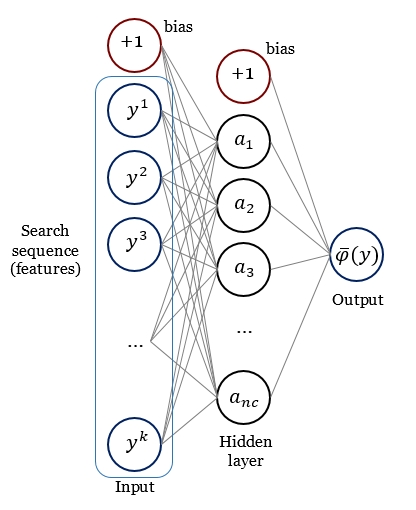
\includegraphics[width=5 cm]{perceptron.jpg}
\caption{Three-layer perceptron with scalar output.\label{fig1}}
\end{center}
\end{figure}
\unskip

The left layer called the input layer consists of a set of neurons $y_i, \; i=\overline{1,k}$ representing the input signals (the values of variables). Each neuron in the hidden layer transforms the values from the previous layer with weighted linear summing 
\begin{linenomath}
\begin{equation}
w_1 y_1 + w_2 y_2+...+w_k y_k+bias,
\end{equation}
\end{linenomath}
where $w_i$ are the weights of the neurons and $bias$ is a special weight, which doesn't include a factor in the form of an input value. Next, the value obtained is transformed into an output (predicted) value of the layer with a transmission function (the \textit{activation function}). The output layer receives the values from the last hidden layer and transforms them into the output values. The network was trained by the error backpropagation method.

We used a three-layered neural network for solving the approximation problem due to the following reasons. From the theoretical point of view, such a network will be sufficient to approximate the function with a high accuracy. From the practical point of view, the use of deep neural networks here will be redundant, because the set of trial results used to build the approximation is small and will not be sufficient to train a deep network.

\subsubsection{Selection of the Model Parameters}

The choice of the solver, the activation function, the value of the regularization parameter, the number of neurons in the hidden layer, etc. are the variable adjustment parameters of the neural network.
For example, for small sets of the multidimensional data, the ``lbfgs'' solver was demonstrated to be better and faster. This solver is a modification of the Broyden-Fletcher-Goldfarb-Shanno algorithm \cite{Nocedal2006} and belongs to the quasi-Newton methods. All numerical experiments were carried out using this algorithm.
The sigmoidal functions (logistic or hyperbolic tangent) were used as the neuron activation functions.
The number of neurons in each layer and the regularization parameter (alpha) were adjusted in the experiments and depended on a particular problem.

In the experiments conducted, we chose the following network architecture:

\begin{verbatim}
    model = MLPRegressor(activation='logistic',
	solver='lbfgs',
	alpha=0.001,
	hidden_layer_sizes=(20,),
	max_iter=5000,
	tol=10e-6,
	random_state=10)
\end{verbatim}


\subsection{The Use of Approximations in Solving the Optimization Problem}\label{GSA_Appr}

In the present study, we applied the following method of using the objective function approximation in the optimization problems: to construct the objective function approximation using the accumulated search information, to find the minimum of the approximation, and to repeat this process either until the computation resources are exhausted or until the convergence is achieved.

The method proposed will make sense either in the case when the amount of the search information accumulated is large enough (that allows constructing a relatively precise approximation of a multiextremal function) or in the case when the problem is similar to a local extremum search problem.
The first case corresponds to the final stage of search and can be interpreted as a method of refining the current solution. However, if the objective function is time-consuming, it is impossible to conduct a large enough number of trials. This is where we will encounter an exhaustion of computing resources.

The second case implies constructing a good approximation based on a relatively small number of trials and in fact includes an assumption on a weak muliextremality of the objective function that matches well with the problem considered within the framework of the present study.
 
The global search algorithm using the objective function approximation can be formulated as follows.
Let us assume that the available resources allow for $K_{max} = K_1 + K_2$ trials to be performed.

At the first stage, $k = K_1$ trials are performed using the core global search algorithm from section \ref{GSA}.
In the course of performing the first stage, a set of the trial results $\Omega = \left\{(y^k, \varphi(y^k)), 0\leq k\leq K_1\right\}$ necessary to construct the objective function approximation is accumulated.

At the second stage, the algorithm works using the approximation. To compute the point $y^{k+1}$ of the next $(k+1)^{\rm th}$ trial, the following operations are performed.

%Описание работы алгоритма
Step 1. Using the set of the trial results $\Omega$ formed in the course of the algorithm execution, to construct an approximation of the objective function $\overline{\varphi}(y)$;

Step 2. Using the core global search algorithm from section \ref{GSA} to find the global minimum of the function $\overline{\varphi}(y)$ and to use this value as the next trial point i. e. $y^{k+1} = \arg \min_{y \in D} \overline{\varphi}(y)$.

Step 3. If either the condition $k>K_{max}$ or the condition $\left\|y^k - y^{k+1}\right\| \leq \epsilon$ is satisfied, to stop the algorithm.
Else, to perform the trial at the point $y^{k+1}$, to store its result in the set $\Omega$, to increment the trial counter $k = k+1$, and to proceed to Step 1.

The algorithm proposed here ensures the convergence to the global solution in the case if $K_1$ trials executed at the first stage are sufficient to construct an approximation of the objective function reflecting the main features of its behavior adequately.

%пример работы алгоирмта на тестовой задаче?

%%%%%%%%%%%%%%%%%%%%%%%%%%%%%%%%%%%%%%%%%%

%\subsection{Loss function definition}

%%%%%%%%%%%%%%%%%%%%%%%%%%%%%%%%%%%%%%%%%%
\section{Results}

%Описание оборудования и программного обеспечения, которое было задействовано при проведении экспериментов.

%Результаты расчетов

%Иллюстрации

%Сравнение нескольких разных решений (это можно перенести и в следующую секцию)

The simulations were conducted using the supercomputer of Lobachevsky University of Nizhni Novgorod (operated under the Linux CentOS 7.2 operation system). Each supercomputer node included two Intel Sandy Bridge E5-2660 2.2 GHz processors, 64 Gb RAM. The central processor unit had 8 cores. 
The global optimization methods considered in the present work were implemented in C++ using GCC 5.5.0 compiler and Open MPI v4.1.1. To construct the objective function approximations using a neural network, scikit-learn machine learning library from Python 3.9 was applied. 
To numerically solve the problem described in Section \ref{math_model}, the open source CFD software OpenFOAM v2012 \cite{OpenFOAM} was used.

%В процессе оптимизации исследовались такие константы, как $\beta^*$, $a_1$, $\alpha_{k 1,2}$, $\alpha_{\omega 1,2}$, которые регулируют скорость диссипации турбулентной кинетической энергии, напряжения Рейнольдса, поток диффузии турбулентной кинетической энергии, поток диффузии диссипации турбулентной кинетической энергии, соответственно.
Such constants of the turbulence model as $\beta^*$, $a_1$, $\alpha_{k 1,2}$, $\alpha_{\omega 1,2}$ have been optimized. They regulate the turbulent kinetic energy dissipation rate, the Reynolds stress, the turbulent kinetic energy diffusion flux, the diffusion flux of turbulent kinetic energy dissipation, respectively.

%Начальные значения коэффициентов были заданы следующими:
The initial values of the coefficients are

\begin{linenomath}
\begin{equation}
	\begin{aligned}
		\beta^* = 0.09;\ \ \ a_1 = 0.31;\ \ \ \alpha_{k 1} = 0.85;\ \ \ \alpha_{\omega 1} = 0.5; \ \ \ \alpha_{k 2} = 1.0;\ \ \ \alpha_{\omega 2} = 0.856.
	\end{aligned}
\end{equation}
\end{linenomath}

One calculation of the objective function for given values of parameters took 15 minutes in average with the use of 8 MPI-processes per node. 

The optimal values of parameters were adjusted for pairs, the values of the remaining parameters were fixed. 
First, a pair of the most important parameters $\beta^*$ and $a_1$ was selected. 
To investigate the optimization problem posed, both possible approaches to solving it were applied: without the use of the objective function approximation  and with the use of the approximation.

In the first experiment, the global search algorithm described in subsection \ref{GSA} was applied without the use of approximation. 
The parameters of the method were set as follows: $r = 3$ and $\epsilon = 10^{-3}$. 
In 24 hours, 100 iterations of the algorithm were performed; the required accuracy was not achieved. 

In the second experiment, the approach described in subsection \ref{GSA_Appr} was applied to solve the same problem.
First, $K_1 = 30$ iterations of global search algorithm were performed. 
Afterwards, the algorithm employing the approximation with the neural network was started. 
A total of $K_1 + K_2 = 65$ iterations of the algorithm were performed, after that the algorithm stopped on accuracy. 
As a result, the best value  of the objective function 0.375 was found. 
The total search time was reduced to 16 hours, which ensured a more accurate solution for the problem in a reasonable amount of time.

The trial points and the approximating function plotted according to these points using the neural network are presented in Figure~\ref{NN_100_point} (the parameters $\beta^*$ and $a_1$ were varied). Several local minima are clearly visible.

\begin{figure}[H]
\begin{center}
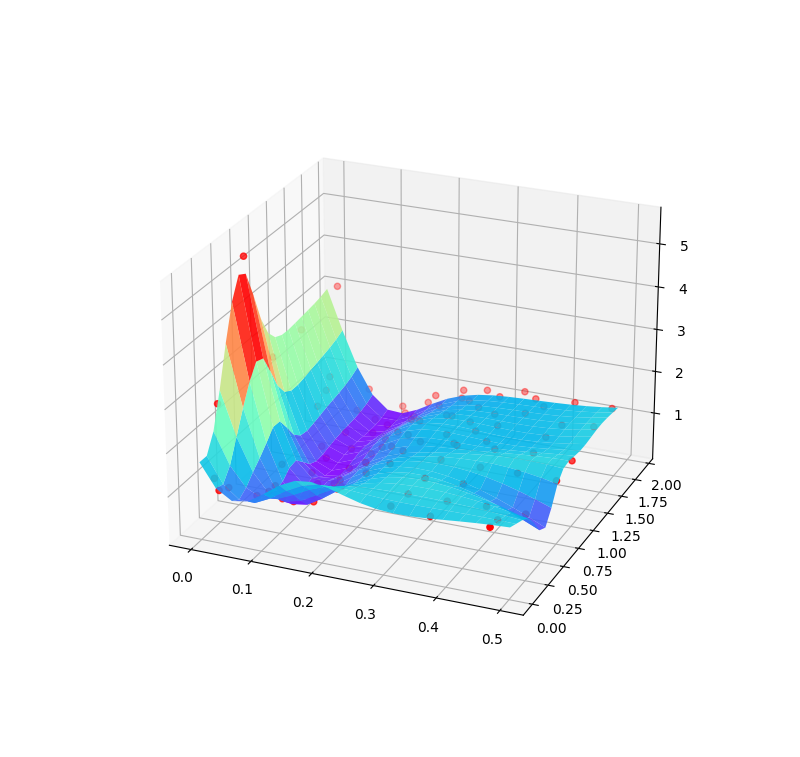
\includegraphics[width=10.5 cm]{NN_100_point_.png}
\caption{Objective function values (red points) and the approximation plot constructed using the neural network (parameters $\beta^*$ and $a_1$ were varied).\label{NN_100_point}}
\end{center}
\end{figure}   
\unskip

The best values of parameters $\beta^*$ and $a_1$ found were fixed, and then optimization in parameters $\alpha_{k1}, \alpha_{\omega1}$, and $\alpha_{k2}, \alpha_{\omega2}$ was performed. 
However, no significant improvement of the objective function by optimizing on these parameters was achieved: the value of 0.365 was obtained.


%На рисунках ~\ref{NN_100_point1} и ~\ref{NN_100_point2} приведены изображение функций, полученные с помощью аппроксимации задачи нейросетью, обученной на 100 точках испытания, варьировались соответсвенно пары параметров $\alpha_{k1} $,  $\alpha_{\omega1} $ и $\alpha_{k2} $, $\alpha_{\omega2} $.
%
%\begin{figure}[H]
%\begin{center}
%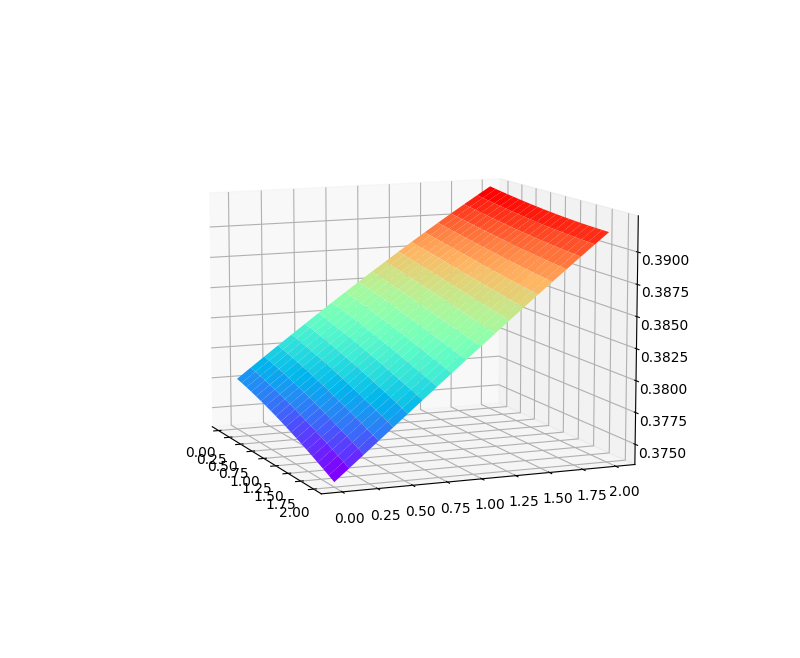
\includegraphics[width=1.0\linewidth]{ NN_100_point_1.png}
%\caption{Изображение функции, полученной с помощью аппроксимации задачи нейросетью, обученной на 100 точках испытания, варьировались параметры $\alpha_{k1} $ и $\alpha_{\omega1} $}
%\label{NN_100_point1}
%\end{center}
%\end{figure}
%
%\begin{figure}[H]
%\begin{center}
%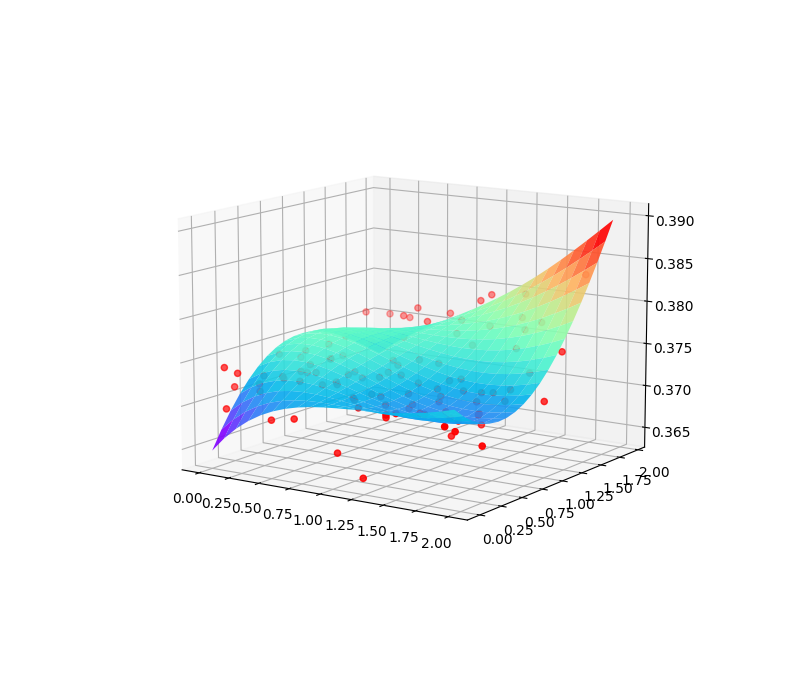
\includegraphics[width=1.0\linewidth]{ NN_100_point_tanh_alpha2_0.0001_.png}
%\caption{Изображение функции, полученной с помощью аппроксимации задачи нейросетью, обученной на 100 точках испытания, варьировались параметры $\alpha_{k2} $ и $\alpha_{\omega2} $}
%\label{NN_100_point2}
%\end{center}
%\end{figure}

%После калибровки значения коэффициентов стали следующими:
%The optimized values of the coefficients:
As a final result, the following values of the coefficients of the model were obtained:

\begin{linenomath}
\begin{equation}
	\begin{aligned}
		\beta^* = 0.117;\ \ \ a_1 = 1.84;\ \ \ \alpha_{k 1} = 1.999;\\
		\alpha_{\omega 1} = 0.062; \ \ \ \alpha_{k 2} = 1.241;\ \ \ \alpha_{\omega 2} = 0.003.
	\end{aligned}
\end{equation}
\end{linenomath}

%Были получены следующие профили скорости на выходной плоскости для различных углов наклона лотка, как показано на рис.~\ref{NIIMexUProfilesKWSSTGlob}
Figure~\ref{NIIMexUProfilesKWSSTGlob} shows the resulting velocity profiles $\bar{\boldsymbol{u_x}}$ as a function from flow depth $h$ on the exit plane for various slope angles.

\begin{figure}[H]
\begin{adjustwidth}{-\extralength}{0cm}
\centering
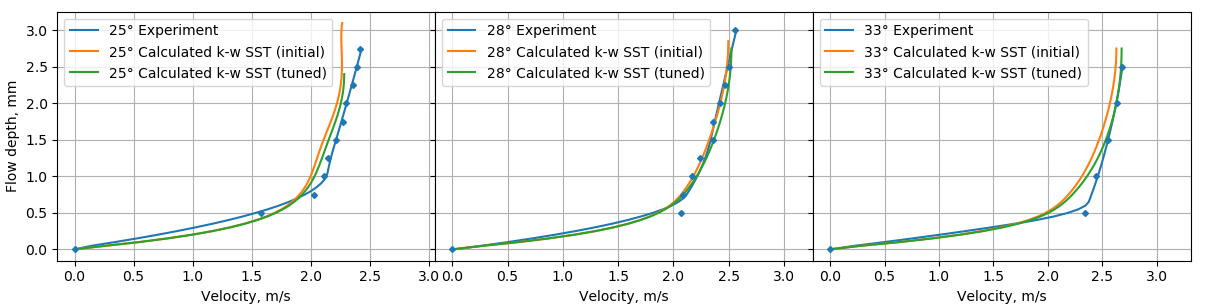
\includegraphics[width=18 cm]{UProfilesKWSSTGlob1.png}
\end{adjustwidth}
\caption{The comparison graphs of the experimental velocity profile and the calculated velocity profile using the standard values of the $k-\omega\ SST$ turbulence model coefficients and the calculated velocity profile with calibrated values of the coefficients for different slope inclination angles.\label{NIIMexUProfilesKWSSTGlob}}
\end{figure}  

%Калибровка привела к следующей минимизации функции потерь~\eqref{LossFunction}, показанной в таб.~\ref{tabLossFunctionMinimize}
During the process of calibration, the minimization of the loss function~\eqref{LossFunction} was achieved the value, as shown in Table~\ref{tabLossFunctionMinimize}.

%\begin{table}[H]
%	\caption{Минимизация функции потерь}
%	\label{tabLossFunctionMinimize}
%	\begin{center}
%		\begin{tabular}{ | c | m{0.3\textwidth} | m{0.3\textwidth} | } 
%			\hline
%			Угол наклона лотка& Начальное значение функции потерь & Минимизированное значение функции потерь\\
%			\hline
%			25$^\circ$ & 0.165 & 0.155\\
%			\hline
%			28$^\circ$ & 0.085 & 0.128\\
%			\hline
%			33$^\circ$ & 0.150 & 0.089\\
%			\hline
%		\end{tabular}
%	\end{center}
%\end{table}
\begin{table}[H] 
\caption{Loss function values obtained during the minimization process.\label{tabLossFunctionMinimize}}
\newcolumntype{C}{>{\centering\arraybackslash}X}
\begin{tabularx}{\textwidth}{CCC}
\toprule
    \textbf{Slope inclination angle} & \textbf{Initial loss function value} & \textbf{Minimized loss function value}\\
\midrule
    25$^\circ$ & 0.165 & 0.155\\
    28$^\circ$ & 0.085 & 0.128\\
    33$^\circ$ & 0.150 & 0.089\\
\bottomrule
\end{tabularx}
\end{table}
\unskip

%На рисунке \ref{NIIMexUProfilesKWSSTGlob} и в таблице \ref{tabLossFunctionMinimizeKE} можем видеть, что для двух углов наклона из трёх мы видим уменьшение расхождения расчётного профиля скорости с экспериментальным. Оптимизация по трём экспериментам одновременно (их функции потерь суммировались) использовалась с целью избежать переобучения модели, так как при использовании одного эксперимента, может быть достигнуто почти идеальное совпадение расчётного профиля скорости с экспериментальным, которое не воспроизводится на других экспериментах. Так же стоит отметить, что расхождение профиля скорости в области вблизи дна обусловлено погрешностью измерений в эксперименте, так как замер скорости с помощью трубки Пито, используемой в данном эксперименте, в непосредственной близости ото дна затруднён.
Figure~\ref{NIIMexUProfilesKWSSTGlob} and Table~\ref{tabLossFunctionMinimize} show a decrease in the discrepancy between the calculated velocity profile and the experimental one for two out of three experiments. Optimization for the three experiments combined (their loss functions were summarized) was used in order to avoid the model overfitting. In one experiment, an almost perfect coincidence of the calculated velocity profile with the experimental one was achieved, which was not reproduced in other experiments. It should also be noted that the divergence of the velocity profile in the region near the chute bottom is due to the measurement error in the experiment, since it is difficult to measure the velocity with the Pitot tube used in this experiment in the immediate vicinity of the bottom.


%%%%%%%%%%%%%%%%%%%%%%%%%%%%%%%%%%%%%%%%%%
\section{Conclusions}

In this work, a two-phase flow in a chute was simulated using the interFoam solver, the URANS mathematical model, and the $k-\omega\ SST$ turbulence model. In the optimization process, six constants were investigated in pairs, which make the greatest contribution to the value of turbulent viscosity.

The results of calculating the velocity profiles were compared with experimental data obtained at the Research Institute of Mechanics, Moscow State University, at different sections depending on the angle of inclination of the chute. The search for the optimal coefficients of the turbulence model was performed by minimizing the objective function of the divergence of the velocity profile in the chute. % - RMSE.

The search for the global minimum of the objective function was performed using the global search algorithm implemented in the Globalizer software \cite{globalizerSystem}. In addition, a fully connected neural network with one hidden layer was used to approximate the values of the objective function by the values of the constants in the turbulence model. The MLPRegressor class from the scikit-learn library was used to build the objective function approximation. 

In the present work, an interdisciplinary approach was utilized, which helped us to find the optimal values of six turbulence model parameters using the OpenFOAM open platform and the Globalizer. The minimum value for the objective function was obtained in the case of the slope angle of 33 degrees. One calculation of the objective function for the given parameters took 15 minutes in average using 8 MPI processes on a node of the Lobachevsky University supercomputer. Total computation time was 24 hours.  

In the future, it is planned to continue improving the turbulent models. Including the creation of a turbulent model based on a neural network. The Globalizer software will be used to optimize the model parameters.

%%%%%%%%%%%%%%%%%%%%%%%%%%%%%%%%%%%%%%%%%%
\vspace{6pt} 

%%%%%%%%%%%%%%%%%%%%%%%%%%%%%%%%%%%%%%%%%%
%% optional
%\supplementary{The following supporting information can be downloaded at:  \linksupplementary{s1}, Figure S1: title; Table S1: title; Video S1: title.}

% Only for the journal Methods and Protocols:
% If you wish to submit a video article, please do so with any other supplementary material.
% \supplementary{The following supporting information can be downloaded at: \linksupplementary{s1}, Figure S1: title; Table S1: title; Video S1: title. A supporting video article is available at doi: link.}

%%%%%%%%%%%%%%%%%%%%%%%%%%%%%%%%%%%%%%%%%%
\authorcontributions{Conceptualization, K.B. and R.D.; methodology, Rom.D. and K.B.; software, I.L., R.D., M.U. and  Rom. D.; validation,  Rom.D. and I.L.; formal analysis, S.S., M.U.; investigation, S.S.; resources, I.L.; data curation, Rom.D. and M.U.; writing---original draft preparation, K.B., S.S. and Rom.D.; writing---review and editing, R.D.; visualization, I.L.; supervision, S.S.; project administration, K.B.; funding acquisition, S.S. All authors have read and agreed to the published version of the manuscript.}

\funding{This research was supported by the Ministry of Science and Higher Education of the Russian Federation, agreement No 075-15-2020-808.}

\institutionalreview{Not applicable.}

\informedconsent{Not applicable.}

\dataavailability{Not applicable.} 

\acknowledgments{The authors consider it their duty to acknowledge the contribution of Prof. Victor Gergel (14.01.1955 -- 29.06.2021), who initiated this interdisciplinary study.}

\conflictsofinterest{The authors declare no conflict of interest.} 

%%%%%%%%%%%%%%%%%%%%%%%%%%%%%%%%%%%%%%%%%%
%% Optional
%\sampleavailability{Samples of the compounds ... are available from the authors.}

%% Only for journal Encyclopedia
%\entrylink{The Link to this entry published on the encyclopedia platform.}

%\abbreviations{Abbreviations}{
%The following abbreviations are used in this manuscript:\\

%\noindent 
%\begin{tabular}{@{}ll}
%MDPI & Multidisciplinary Digital Publishing Institute\\
%DOAJ & Directory of open access journals\\
%TLA & Three letter acronym\\
%LD & Linear dichroism
%\end{tabular}
%}

%%%%%%%%%%%%%%%%%%%%%%%%%%%%%%%%%%%%%%%%%%
%% Optional
\appendixtitles{no} % Leave argument "no" if all appendix headings stay EMPTY (then no dot is printed after "Appendix A"). If the appendix sections contain a heading then change the argument to "yes".
\appendixstart
\appendix
\section[\appendixname~\thesection]{}\label{app}%Nomenclature%List of symbols and abbreviations
%\subsection[\appendixname~\thesubsection]{}
%The appendix is an optional section that can contain details and data supplemental to the main text---for example, explanations of experimental details that would disrupt the flow of the main text but nonetheless remain crucial to understanding and reproducing the research shown; figures of replicates for experiments of which representative data are shown in the main text can be added here if brief, or as Supplementary Data. Mathematical proofs of results not central to the paper can be added as an appendix.

\begin{table}[H] 
\caption{Nomenclature.\label{A:tab1}}
\newcolumntype{C}{>{\centering\arraybackslash}X}
\begin{tabularx}{\textwidth}{ll}
\toprule
\textbf{Title 1}	& \textbf{Title 2}	\\
\midrule
$u_0$		& depth-averaged velocity on the inlet plane of experiment chute	\\
$h_0$		& flow depth on the inlet plane of experiment chute	\\
$\theta$	& inclination angle of the experiment chute \\
$\alpha$	& water volume fraction	\\
$\bar{\boldsymbol{\tau}}$	& Reynolds-averaged stress tensor	\\
$\bar{\boldsymbol{s}}$		& Reynolds-averaged strain rate tensor	\\
$\mu_{eff}$		& effective viscosity	\\
$\mu$		& molecular viscosity	\\
$\mu_{t}$		& turbulent viscosity	\\
$\bar{\boldsymbol{f}}$		& Reynolds-averaged density of body forces	\\
$\bar{\boldsymbol{u}}$		& Reynolds-averaged velocity of the mixture	\\
$\rho$		& density of the mixture	\\
$\bar{p}$		& pressure of the mixture	\\
$\omega$		& specific dissipation rate of the turbulent kinetic energy	\\
$k$		& 	turbulent kinetic energy \\
$F_1$		& first blending function	\\
$\dot{\boldsymbol{s}}$		& Reynolds-averaged strain rate (second invariant of the Reynolds-averaged strain rate tensor $\bar{\boldsymbol{s}}$)	\\
$F_2$		& second blending function	\\
$\widetilde{P}_k$ & the limiter on the growth of turbulence used in stagnation modes \\
$\alpha_k$ & turbulence model constant \\
$\alpha_{k1}$ & turbulence model constant \\
$\alpha_{k2}$ & turbulence model constant \\
$\alpha_\omega$ & turbulence model constant \\
$\alpha_{\omega1}$ & turbulence model constant \\
$\alpha_{\omega2}$ & turbulence model constant \\
$\beta$ & turbulence model constant \\
$\beta_1$ & turbulence model constant \\
$\beta_2$ & turbulence model constant \\
$\gamma$ & turbulence model constant \\
$\gamma_1$ & turbulence model constant \\
$\gamma_2$ & turbulence model constant \\
$\beta^*$ & turbulence model constant \\
$a_1$ & turbulence model constant \\
$b_1$ & turbulence model constant \\
$c_1$ & turbulence model constant \\
$y = (y_1, ..., y_N)$ & vector of parameters values\\
$\varphi(y)$		& optimization criterion	\\
$D$	& hyperinterval	\\
$N$		& number of measuring points of velocity over the flow depth at the outlet plane	\\
$u^i_{EXP}$		& horizontal component of velocity at the control point obtained by experiment	\\
$u^i_{k-\omega}\ SST$		& horizontal component of velocity at the control point calculated by CFD	\\
$\boldsymbol{L_{RMSE}}$		& loss function	\\
$L$		& Lipschitz constant	\\
$H$		& H{\"o}lder constant	\\
$f(x)$		& univariate function	\\
Entry 2		& Data	\\
Entry 2		& Data	\\
Entry 2		& Data	\\
Entry 2		& Data	\\
Entry 2		& Data	\\
\bottomrule
\end{tabularx}
\end{table}

\begin{table}[H] 
\caption{List of abbreviation.\label{A:tab2}}
\newcolumntype{C}{>{\centering\arraybackslash}X}
\begin{tabularx}{\textwidth}{ll}
\toprule
\textbf{Title 1}	& \textbf{Title 2}	\\
\midrule
NNR		& Neural Network Regression	\\
RMSE		& Root-Mean-Square Error	\\
CFD & Computational Fluid Dynamic \\
\bottomrule
\end{tabularx}
\end{table}

%\section[\appendixname~\thesection]{}
%All appendix sections must be cited in the main text. In the appendices, Figures, Tables, etc. should be labeled, starting with ``A''---e.g., Figure A1, Figure A2, etc.

%%%%%%%%%%%%%%%%%%%%%%%%%%%%%%%%%%%%%%%%%%
\begin{adjustwidth}{-\extralength}{0cm}
%\printendnotes[custom] % Un-comment to print a list of endnotes

\reftitle{References}

% Please provide either the correct journal abbreviation (e.g. according to the “List of Title Word Abbreviations” http://www.issn.org/services/online-services/access-to-the-ltwa/) or the full name of the journal.
% Citations and References in Supplementary files are permitted provided that they also appear in the reference list here. 

%=====================================
% References, variant A: external bibliography
%=====================================
%\bibliography{your_external_BibTeX_file}
\bibliography{bibliography}

%=====================================
% References, variant B: internal bibliography
%=====================================
%\begin{thebibliography}{999}
% Reference 1
%\bibitem[Author1(year)]{ref-journal}
%Author~1, T. The title of the cited article. {\em Journal Abbreviation} {\bf 2008}, {\em 10}, 142--149.
% Reference 2
%\bibitem[Author2(year)]{ref-book1}
%Author~2, L. The title of the cited contribution. In {\em The Book Title}; Editor 1, F., Editor 2, A., Eds.; Publishing House: City, Country, 2007; pp. 32--58.
% Reference 3
%\bibitem[Author3(year)]{ref-book2}
%Author 1, A.; Author 2, B. \textit{Book Title}, 3rd ed.; Publisher: Publisher Location, Country, 2008; pp. 154--196.
% Reference 4
%\bibitem[Author4(year)]{ref-unpublish}
%Author 1, A.B.; Author 2, C. Title of Unpublished Work. \textit{Abbreviated Journal Name} year, \textit{phrase indicating stage of publication (submitted; accepted; in press)}.
% Reference 5
%\bibitem[Author5(year)]{ref-communication}
%Author 1, A.B. (University, City, State, Country); Author 2, C. (Institute, City, State, Country). Personal communication, 2012.
% Reference 6
%\bibitem[Author6(year)]{ref-proceeding}
%Author 1, A.B.; Author 2, C.D.; Author 3, E.F. Title of presentation. In Proceedings of the Name of the Conference, Location of Conference, Country, Date of Conference (Day Month Year); Abstract Number (optional), Pagination (optional).
% Reference 7
%\bibitem[Author7(year)]{ref-thesis}
%Author 1, A.B. Title of Thesis. Level of Thesis, Degree-Granting University, Location of University, Date of Completion.
% Reference 8
%\bibitem[Author8(year)]{ref-url}
%Title of Site. Available online: URL (accessed on Day Month Year).
%\end{thebibliography}

% If authors have biography, please use the format below
%\section*{Short Biography of Authors}
%\bio
%{\raisebox{-0.35cm}{\includegraphics[width=3.5cm,height=5.3cm,clip,keepaspectratio]{Definitions/author1.pdf}}}
%{\textbf{Firstname Lastname} Biography of first author}
%
%\bio
%{\raisebox{-0.35cm}{\includegraphics[width=3.5cm,height=5.3cm,clip,keepaspectratio]{Definitions/author2.jpg}}}
%{\textbf{Firstname Lastname} Biography of second author}

% For the MDPI journals use author-date citation, please follow the formatting guidelines on http://www.mdpi.com/authors/references
% To cite two works by the same author: \citeauthor{ref-journal-1a} (\citeyear{ref-journal-1a}, \citeyear{ref-journal-1b}). This produces: Whittaker (1967, 1975)
% To cite two works by the same author with specific pages: \citeauthor{ref-journal-3a} (\citeyear{ref-journal-3a}, p. 328; \citeyear{ref-journal-3b}, p.475). This produces: Wong (1999, p. 328; 2000, p. 475)

%%%%%%%%%%%%%%%%%%%%%%%%%%%%%%%%%%%%%%%%%%
%% for journal Sci
%\reviewreports{\\
%Reviewer 1 comments and authors’ response\\
%Reviewer 2 comments and authors’ response\\
%Reviewer 3 comments and authors’ response
%}
%%%%%%%%%%%%%%%%%%%%%%%%%%%%%%%%%%%%%%%%%%
\end{adjustwidth}
\end{document}

